%
% 計測自動制御学会システム・情報部門学術講演会2013原稿サンプルファイル
%                                           August 26, 2013
% 計測自動制御学会システム・情報部門学術講演会2011原稿サンプルファイル
%                                           April 28, 2011
% Based on 第7回計測自動制御学会制御部門大会原稿サンプルファイル
%                                           October 18, 2007
% Based on 第5回計測自動制御学会制御部門大会原稿サンプルファイル
%            近野敦 konno@space.mech.tohoku.ac.jp    March 05, 2005
%
% LaTeX2eとLaTeX209判別のための定義(以下3行)は科研費マクロkkhgrp.mac
% の定義を,作者の金沢大学青木先生の許可を得て利用させていただきました.
%
\newif\ifLaTeXe\LaTeXefalse
\expandafter\ifx\csname PackageError\endcsname\relax\LaTeXefalse
\else\LaTeXetrue\fi

\ifLaTeXe
  \documentclass{jarticle}
  \usepackage{SICE-SSI}
  \usepackage[dvips]{graphicx}
\else
  \documentstyle[SICE-SSI,epsbox]{jarticle}
\fi

\begin{document}
\title{UPPAALによる交差点における自動運転車群のモデル化と検証}
\author{○佐原優衣\ 中村正樹\ 榊原一紀\ 玉置久\ (富山県立大学)}

\abstract{
  この原稿のサンプルには,SSI2015 の原稿執筆およびアップロードにおける注意が
  記されています.
  電子投稿システムではPDFファイルのみ受け付けます.
  }

\keyword{自動運転車制御,形式検証,時間オートマトン,UPPAAL}

\maketitle\thispagestyle{empty}
\pagestyle{empty}

\section{はじめに}
近年,自動運転技術が急速に発達している. 自動運転は,搭載される技術によってレベル1からレベル5までに分けられており,現在,日本国内では,運転者支援を主としたレベル2までが市販車に採用されている.今後,高速道路や,限定地域での特定条件下での完全自動運転を行うレベル4の車両の普及が目指されている.
自動運転技術が普及し,大量の自動運転車が利用される都市空間を考える.
道路上の車両密度が高くなるため,渋滞やデッドロックが発生することが想定される.したがって,個々の車両だけではなく,自動運転車群が効率的に走行するアルゴリズムが必要となる.
	
本研究では群制御アルゴリズムが安全性に関わる衝突回避やデッドロック回避,効率性に関わる時間制約などの性質を満たすかどうかを検証する手法を提案する.
自動運転車の群制御アルゴリズムを形式的に記述し,モデル検査を用いて,性質を検証する.モデル検査は,システム上で起こり得る状態を網羅的に調べることにより設計の誤りを発見する自動検証手法の一種である.モデル検査手法は,システムの振る舞いの設計,および検証したい性質をそれぞれモデル化し,ツールを用いて,システムが性質を満たしているかを調べる.
本研究では,時間オートマトン\cite{u3}による時間制約検証が行えるモデル検査ツールUPPAAL\cite{u1,u2}を採用する.
UPPAALを用いて交差点を通過する1台の自動運転車の挙動をモデル化する。交差点は2車線対面通行で右折用レーンはなく,信号もない交差点とする.

\section{テンプレートファイルのダウンロード}

SSI2015のホームページ\cite{大会ホームページ}
からテンプレートファイルをダウンロードします.pLaTeX2.09またはpLaTeX2e
を使用される場合は,SICE-SSI.styとsample.texの二つのファイルをダウンロ
ードしてください.sample.texはpLaTeX2eとpLaTeX2.09のどちらでもコンパイ
ルすることができます.SICE-SSI.styとsample.texはUTF8版,SJIS版,EUC版の3種類を
用意しましたので,それぞれの環境に応じてダウンロードするファイルを選択
してください.Microsoft Word(以下MS-Wordと略す)を使用される場合は,
template.docをダウンロードし,原稿を作成してください.それ以外のワード
プロセッサをご使用の方は,sample.pdfをダウンロードし,原稿の体裁がなるべ
くサンプルと近くなるよう原稿を作成ください.

\section{原稿の体裁}

原稿は1ページ以上6ページ以下です.
アップロードするファイルサイズに特に制限は設けませんが,
あまりに巨大である場合,ファイルサイズの縮小をお願いする場合があります.

\subsection{全体の体裁}

A4用紙の(US Letterは不可),縦250 mm,横170 mmの枠内に収まるようにし
てください.余白は,上20 mm,下27 mm,左20 mm,右20 mmとします.活字の
大きさは,題目16ポイント,著者名と所属12ポイント,概要とキーワード9ポイ
ント,章タイトル11ポイント,節タイトル10ポイント,本文の活字10ポイント,
参考文献9ポイントを目安としてください.原稿は,
%
\begin{itemize}
  \setlength{\topsep}{0pt}
  \setlength{\partopsep}{0pt}
  \setlength{\itemsep}{0pt}
  \setlength{\parsep}{0pt}
  \setlength{\parskip}{1pt plus 1pt minus 1pt}
  \item 題目
  \item 著者名(登壇者に○印)と所属
  \item 概要
  \item キーワード
  \item 本文,参考文献
\end{itemize}
%
の順に書いてください.キーワードまでを1段組,本文・参考文献を2段組にしてください. 

\subsection{図と表}

\begin{figure}[t]
  \centering
\ifLaTeXe
  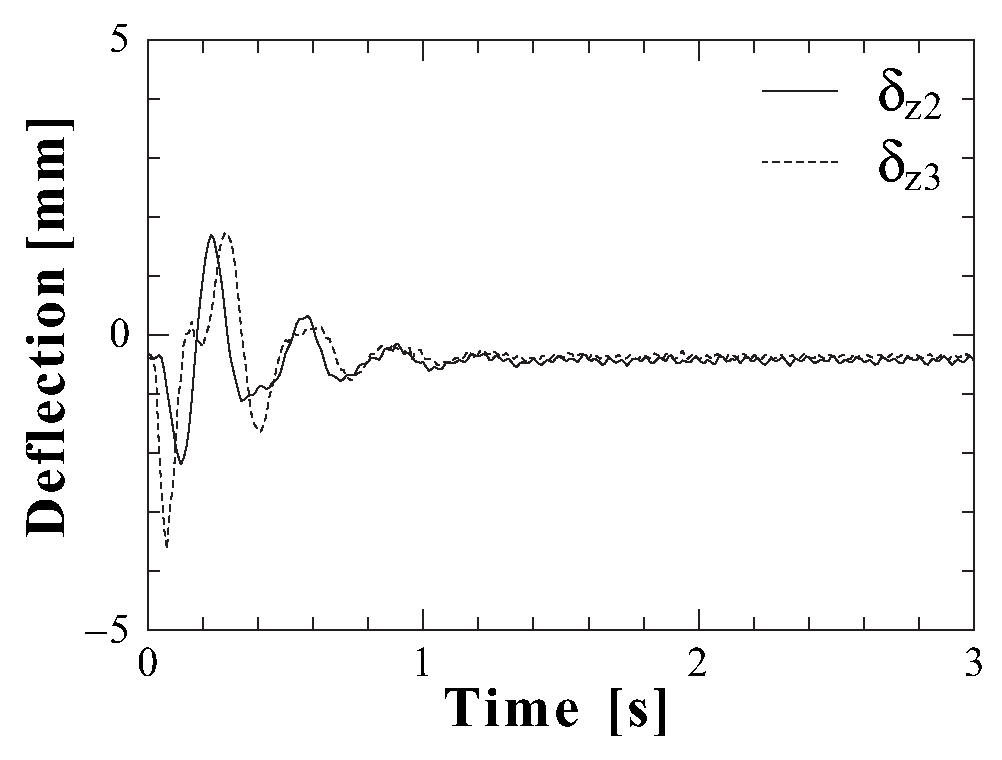
\includegraphics[width=0.5\linewidth]{fig1}
\else
  \psbox[width=0.55\linewidth]{fig1}
\fi
  \caption{A sample figure.}
  \label{fig:samplefig}
\end{figure}

図と表は,Fig.~1,Table~1のように番号を振り
(Fig.~\ref{fig:samplefig}\ 参照),図説,図中の
説明文は英文で記入してください.本文で引用する場合も「Fig.~1に示す」な
どのようにFig.とTableを使用してください.

図や表中の文字は小さくなりすぎないよう気をつけてください.PDF原稿を作
成する際,図の画質が落ちないよう,注意してください.特にMicrosoft Word
などで原稿を作成する際,JPEG画像を貼り付けると,一度圧縮されている画像
が再圧縮されるので画像が劣化するようです.貼り付ける画像は,画質の良い
(圧縮率の低い)画像を用いるか圧縮しない画像フォーマットを選ぶなど,各
自工夫し,最終的なPDFファイルにおいて画像が劣化しないよう注意してくだ
さい.

\subsection{参考文献}

文献の引用は本文中に\cite{大会ホームページ}のように書き,本文の最後に
まとめて記述します.次のフォーマットを推奨します.

\noindent
(a) 雑誌論文の場合

\noindent
番号)  著者:論文題目,雑誌名,巻(太字)-号,始ページ/終ページ(年)

\noindent
(b) 単行本の場合

\noindent
番号)  著者:書名,始ページ/終ページ,発行所(発行年)

なお,本研究が他学会で発表済みの内容の場合,その文献を参考文献に挙げるとともに,脚注で明示して下さい.

\small
\begin{thebibliography}{3}
%%%%%%%%%%%%%%%%%%%%%%%%%%%%%%%%%%%%%%%%%%%%%%%%%%%%%%%%%%%%%%%%%%%%%%%%%%%%%%%

\bibitem{u1}{Kim Guldstrand Larsen and Paul Pettersson and Wang Yi, UPPAAL in a Nutshell, International Journal of Software Tools for Technology Transfer, Vol.1, No.1-2, pp.134-152, 1997.}
\bibitem{u2}{UPPAAL, \verb$http://www.uppaal.org$}
\bibitem{u3}{Johan BengtssonWang Yi, Timed Automata: Semantics, Algorithms and Tools,  Lectures on Concurrency and Petri Nets: Advances in Petri Nets, number 3098 in LNCS, pp.87-124, 2004.}


%%%%%%%%%%%%%%%%%%%%%%%%%%%%%%%%%%%%%%%%%%%%%%%%%%%%%%%%%%%%%%%%%%%%%%%%%%%%%%%
\end{thebibliography}


\end{document}
